\documentclass{beamer}
\usepackage{graphicx, color}

% Use something like:
% % Use something like:
% % Use something like:
% \input{../../macros}

% groupings of objects.
\newcommand{\set}[1]{\left\{ #1 \right\}}
\newcommand{\seq}[1]{\left(#1\right)}
\newcommand{\ang}[1]{\langle#1\rangle}
\newcommand{\tuple}[1]{\left(#1\right)}

% numerical shortcuts.
\newcommand{\abs}[1]{\left| #1\right|}
\newcommand{\floor}[1]{\left\lfloor #1 \right\rfloor}
\newcommand{\ceil}[1]{\left\lceil #1 \right\rceil}

% linear algebra shortcuts.
\newcommand{\change}{\Delta}
\newcommand{\norm}[1]{\left\| #1\right\|}
\newcommand{\dprod}[1]{\langle#1\rangle}
\newcommand{\linspan}[1]{\langle#1\rangle}
\newcommand{\conj}[1]{\overline{#1}}
\newcommand{\gradient}{\nabla}
\newcommand{\der}{\frac{d}{dx}}
\newcommand{\lap}{\Delta}
\newcommand{\kron}{\otimes}
\newcommand{\nperp}{\nvdash}

\newcommand{\mat}[1]{\left( \begin{smallmatrix}#1 \end{smallmatrix} \right)}

% derivatives and limits
\newcommand{\partder}[2]{\frac{\partial #1}{\partial #2}}
\newcommand{\partdern}[3]{\frac{\partial^{#3} #1}{\partial #2^{#3}}}

% Arrows
\newcommand{\diverge}{\nearrow}
\newcommand{\notto}{\nrightarrow}
\newcommand{\up}{\uparrow}
\newcommand{\down}{\downarrow}
% gets and gives are defined!

% ordering operators
\newcommand{\oleq}{\preceq}
\newcommand{\ogeq}{\succeq}

% programming and logic operators
\newcommand{\dfn}{:=}
\newcommand{\assign}{:=}
\newcommand{\co}{\ co\ }
\newcommand{\en}{\ en\ }


% logic operators
\newcommand{\xor}{\oplus}
\newcommand{\Land}{\bigwedge}
\newcommand{\Lor}{\bigvee}
\newcommand{\finish}{$\Box$}
\newcommand{\contra}{\Rightarrow \Leftarrow}
\newcommand{\iseq}{\stackrel{_?}{=}}


% Set theory
\newcommand{\symdiff}{\Delta}
\newcommand{\union}{\cup}
\newcommand{\inters}{\cap}
\newcommand{\Union}{\bigcup}
\newcommand{\Inters}{\bigcap}
\newcommand{\nullSet}{\phi}

% graph theory
\newcommand{\nbd}{\Gamma}

% Script alphabets
% For reals, use \Re

% greek letters
\newcommand{\eps}{\epsilon}
\newcommand{\del}{\delta}
\newcommand{\ga}{\alpha}
\newcommand{\gb}{\beta}
\newcommand{\gd}{\del}
\newcommand{\gf}{\phi}
\newcommand{\gF}{\Phi}
\newcommand{\gl}{\lambda}
\newcommand{\gm}{\mu}
\newcommand{\gn}{\nu}
\newcommand{\gr}{\rho}
\newcommand{\gs}{\sigma}
\newcommand{\gt}{\theta}
\newcommand{\gx}{\xi}

\newcommand{\sw}{\sigma}
\newcommand{\SW}{\Sigma}
\newcommand{\ew}{\lambda}
\newcommand{\EW}{\Lambda}

\newcommand{\Del}{\Delta}
\newcommand{\gD}{\Delta}
\newcommand{\gG}{\Gamma}
\newcommand{\gO}{\Omega}
\newcommand{\gL}{\Lambda}
\newcommand{\gS}{\Sigma}

% Formatting shortcuts
\newcommand{\red}[1]{\textcolor{red}{#1}}
\newcommand{\blue}[1]{\textcolor{blue}{#1}}
\newcommand{\htext}[2]{\texorpdfstring{#1}{#2}}

% Statistics
\newcommand{\distr}{\sim}
\newcommand{\stddev}{\sigma}
\newcommand{\covmatrix}{\Sigma}
\newcommand{\mean}{\mu}
\newcommand{\param}{\gt}
\newcommand{\ftr}{\phi}

% General utility
\newcommand{\todo}[1]{\footnote{TODO: #1}}
\newcommand{\exclaim}[1]{{\textbf{\textit{#1}}}}
\newcommand{\tbc}{[\textbf{Incomplete}]}
\newcommand{\chk}{[\textbf{Check}]}
\newcommand{\oprob}{[\textbf{OP}]:}
\newcommand{\core}[1]{\textbf{Core Idea:}}
\newcommand{\why}{[\textbf{Find proof}]}
\newcommand{\opt}[1]{\textit{#1}}


\DeclareMathOperator*{\argmin}{arg\,min}
\DeclareMathOperator{\rank}{rank}
\newcommand{\redcol}[1]{\textcolor{red}{#1}}
\newcommand{\bluecol}[1]{\textcolor{blue}{#1}}
\newcommand{\greencol}[1]{\textcolor{green}{#1}}


\renewcommand{\~}{\htext{$\sim$}{~}}


% groupings of objects.
\newcommand{\set}[1]{\left\{ #1 \right\}}
\newcommand{\seq}[1]{\left(#1\right)}
\newcommand{\ang}[1]{\langle#1\rangle}
\newcommand{\tuple}[1]{\left(#1\right)}

% numerical shortcuts.
\newcommand{\abs}[1]{\left| #1\right|}
\newcommand{\floor}[1]{\left\lfloor #1 \right\rfloor}
\newcommand{\ceil}[1]{\left\lceil #1 \right\rceil}

% linear algebra shortcuts.
\newcommand{\change}{\Delta}
\newcommand{\norm}[1]{\left\| #1\right\|}
\newcommand{\dprod}[1]{\langle#1\rangle}
\newcommand{\linspan}[1]{\langle#1\rangle}
\newcommand{\conj}[1]{\overline{#1}}
\newcommand{\gradient}{\nabla}
\newcommand{\der}{\frac{d}{dx}}
\newcommand{\lap}{\Delta}
\newcommand{\kron}{\otimes}
\newcommand{\nperp}{\nvdash}

\newcommand{\mat}[1]{\left( \begin{smallmatrix}#1 \end{smallmatrix} \right)}

% derivatives and limits
\newcommand{\partder}[2]{\frac{\partial #1}{\partial #2}}
\newcommand{\partdern}[3]{\frac{\partial^{#3} #1}{\partial #2^{#3}}}

% Arrows
\newcommand{\diverge}{\nearrow}
\newcommand{\notto}{\nrightarrow}
\newcommand{\up}{\uparrow}
\newcommand{\down}{\downarrow}
% gets and gives are defined!

% ordering operators
\newcommand{\oleq}{\preceq}
\newcommand{\ogeq}{\succeq}

% programming and logic operators
\newcommand{\dfn}{:=}
\newcommand{\assign}{:=}
\newcommand{\co}{\ co\ }
\newcommand{\en}{\ en\ }


% logic operators
\newcommand{\xor}{\oplus}
\newcommand{\Land}{\bigwedge}
\newcommand{\Lor}{\bigvee}
\newcommand{\finish}{$\Box$}
\newcommand{\contra}{\Rightarrow \Leftarrow}
\newcommand{\iseq}{\stackrel{_?}{=}}


% Set theory
\newcommand{\symdiff}{\Delta}
\newcommand{\union}{\cup}
\newcommand{\inters}{\cap}
\newcommand{\Union}{\bigcup}
\newcommand{\Inters}{\bigcap}
\newcommand{\nullSet}{\phi}

% graph theory
\newcommand{\nbd}{\Gamma}

% Script alphabets
% For reals, use \Re

% greek letters
\newcommand{\eps}{\epsilon}
\newcommand{\del}{\delta}
\newcommand{\ga}{\alpha}
\newcommand{\gb}{\beta}
\newcommand{\gd}{\del}
\newcommand{\gf}{\phi}
\newcommand{\gF}{\Phi}
\newcommand{\gl}{\lambda}
\newcommand{\gm}{\mu}
\newcommand{\gn}{\nu}
\newcommand{\gr}{\rho}
\newcommand{\gs}{\sigma}
\newcommand{\gt}{\theta}
\newcommand{\gx}{\xi}

\newcommand{\sw}{\sigma}
\newcommand{\SW}{\Sigma}
\newcommand{\ew}{\lambda}
\newcommand{\EW}{\Lambda}

\newcommand{\Del}{\Delta}
\newcommand{\gD}{\Delta}
\newcommand{\gG}{\Gamma}
\newcommand{\gO}{\Omega}
\newcommand{\gL}{\Lambda}
\newcommand{\gS}{\Sigma}

% Formatting shortcuts
\newcommand{\red}[1]{\textcolor{red}{#1}}
\newcommand{\blue}[1]{\textcolor{blue}{#1}}
\newcommand{\htext}[2]{\texorpdfstring{#1}{#2}}

% Statistics
\newcommand{\distr}{\sim}
\newcommand{\stddev}{\sigma}
\newcommand{\covmatrix}{\Sigma}
\newcommand{\mean}{\mu}
\newcommand{\param}{\gt}
\newcommand{\ftr}{\phi}

% General utility
\newcommand{\todo}[1]{\footnote{TODO: #1}}
\newcommand{\exclaim}[1]{{\textbf{\textit{#1}}}}
\newcommand{\tbc}{[\textbf{Incomplete}]}
\newcommand{\chk}{[\textbf{Check}]}
\newcommand{\oprob}{[\textbf{OP}]:}
\newcommand{\core}[1]{\textbf{Core Idea:}}
\newcommand{\why}{[\textbf{Find proof}]}
\newcommand{\opt}[1]{\textit{#1}}


\DeclareMathOperator*{\argmin}{arg\,min}
\DeclareMathOperator{\rank}{rank}
\newcommand{\redcol}[1]{\textcolor{red}{#1}}
\newcommand{\bluecol}[1]{\textcolor{blue}{#1}}
\newcommand{\greencol}[1]{\textcolor{green}{#1}}


\renewcommand{\~}{\htext{$\sim$}{~}}


% groupings of objects.
\newcommand{\set}[1]{\left\{ #1 \right\}}
\newcommand{\seq}[1]{\left(#1\right)}
\newcommand{\ang}[1]{\langle#1\rangle}
\newcommand{\tuple}[1]{\left(#1\right)}

% numerical shortcuts.
\newcommand{\abs}[1]{\left| #1\right|}
\newcommand{\floor}[1]{\left\lfloor #1 \right\rfloor}
\newcommand{\ceil}[1]{\left\lceil #1 \right\rceil}

% linear algebra shortcuts.
\newcommand{\change}{\Delta}
\newcommand{\norm}[1]{\left\| #1\right\|}
\newcommand{\dprod}[1]{\langle#1\rangle}
\newcommand{\linspan}[1]{\langle#1\rangle}
\newcommand{\conj}[1]{\overline{#1}}
\newcommand{\gradient}{\nabla}
\newcommand{\der}{\frac{d}{dx}}
\newcommand{\lap}{\Delta}
\newcommand{\kron}{\otimes}
\newcommand{\nperp}{\nvdash}

\newcommand{\mat}[1]{\left( \begin{smallmatrix}#1 \end{smallmatrix} \right)}

% derivatives and limits
\newcommand{\partder}[2]{\frac{\partial #1}{\partial #2}}
\newcommand{\partdern}[3]{\frac{\partial^{#3} #1}{\partial #2^{#3}}}

% Arrows
\newcommand{\diverge}{\nearrow}
\newcommand{\notto}{\nrightarrow}
\newcommand{\up}{\uparrow}
\newcommand{\down}{\downarrow}
% gets and gives are defined!

% ordering operators
\newcommand{\oleq}{\preceq}
\newcommand{\ogeq}{\succeq}

% programming and logic operators
\newcommand{\dfn}{:=}
\newcommand{\assign}{:=}
\newcommand{\co}{\ co\ }
\newcommand{\en}{\ en\ }


% logic operators
\newcommand{\xor}{\oplus}
\newcommand{\Land}{\bigwedge}
\newcommand{\Lor}{\bigvee}
\newcommand{\finish}{$\Box$}
\newcommand{\contra}{\Rightarrow \Leftarrow}
\newcommand{\iseq}{\stackrel{_?}{=}}


% Set theory
\newcommand{\symdiff}{\Delta}
\newcommand{\union}{\cup}
\newcommand{\inters}{\cap}
\newcommand{\Union}{\bigcup}
\newcommand{\Inters}{\bigcap}
\newcommand{\nullSet}{\phi}

% graph theory
\newcommand{\nbd}{\Gamma}

% Script alphabets
% For reals, use \Re

% greek letters
\newcommand{\eps}{\epsilon}
\newcommand{\del}{\delta}
\newcommand{\ga}{\alpha}
\newcommand{\gb}{\beta}
\newcommand{\gd}{\del}
\newcommand{\gf}{\phi}
\newcommand{\gF}{\Phi}
\newcommand{\gl}{\lambda}
\newcommand{\gm}{\mu}
\newcommand{\gn}{\nu}
\newcommand{\gr}{\rho}
\newcommand{\gs}{\sigma}
\newcommand{\gt}{\theta}
\newcommand{\gx}{\xi}

\newcommand{\sw}{\sigma}
\newcommand{\SW}{\Sigma}
\newcommand{\ew}{\lambda}
\newcommand{\EW}{\Lambda}

\newcommand{\Del}{\Delta}
\newcommand{\gD}{\Delta}
\newcommand{\gG}{\Gamma}
\newcommand{\gO}{\Omega}
\newcommand{\gL}{\Lambda}
\newcommand{\gS}{\Sigma}

% Formatting shortcuts
\newcommand{\red}[1]{\textcolor{red}{#1}}
\newcommand{\blue}[1]{\textcolor{blue}{#1}}
\newcommand{\htext}[2]{\texorpdfstring{#1}{#2}}

% Statistics
\newcommand{\distr}{\sim}
\newcommand{\stddev}{\sigma}
\newcommand{\covmatrix}{\Sigma}
\newcommand{\mean}{\mu}
\newcommand{\param}{\gt}
\newcommand{\ftr}{\phi}

% General utility
\newcommand{\todo}[1]{\footnote{TODO: #1}}
\newcommand{\exclaim}[1]{{\textbf{\textit{#1}}}}
\newcommand{\tbc}{[\textbf{Incomplete}]}
\newcommand{\chk}{[\textbf{Check}]}
\newcommand{\oprob}{[\textbf{OP}]:}
\newcommand{\core}[1]{\textbf{Core Idea:}}
\newcommand{\why}{[\textbf{Find proof}]}
\newcommand{\opt}[1]{\textit{#1}}


\DeclareMathOperator*{\argmin}{arg\,min}
\DeclareMathOperator{\rank}{rank}
\newcommand{\redcol}[1]{\textcolor{red}{#1}}
\newcommand{\bluecol}[1]{\textcolor{blue}{#1}}
\newcommand{\greencol}[1]{\textcolor{green}{#1}}


\renewcommand{\~}{\htext{$\sim$}{~}}

% Use something like:
% % Use something like:
% % Use something like:
% \input{../../presentationMacros}

% Useful shorthands.
\newcommand{\pitem}{\pause \item}
\AtBeginSection[]
{
   \begin{frame}
       \frametitle{Outline}
       \tableofcontents[currentsection]
   \end{frame}
}

\AtBeginSubsection[]
{
   \begin{frame}
       \frametitle{Outline}
       \tableofcontents[currentsection,currentsubsection]
   \end{frame}
}

\AtBeginSubsubsection[]
{
   \begin{frame}
       \frametitle{Outline}
       \tableofcontents[currentsection,currentsubsection, currentsubsubsection]
   \end{frame}
}


% Useful shorthands.
\newcommand{\pitem}{\pause \item}
\AtBeginSection[]
{
   \begin{frame}
       \frametitle{Outline}
       \tableofcontents[currentsection]
   \end{frame}
}

\AtBeginSubsection[]
{
   \begin{frame}
       \frametitle{Outline}
       \tableofcontents[currentsection,currentsubsection]
   \end{frame}
}

\AtBeginSubsubsection[]
{
   \begin{frame}
       \frametitle{Outline}
       \tableofcontents[currentsection,currentsubsection, currentsubsubsection]
   \end{frame}
}


% Useful shorthands.
\newcommand{\pitem}{\pause \item}
\AtBeginSection[]
{
   \begin{frame}
       \frametitle{Outline}
       \tableofcontents[currentsection]
   \end{frame}
}

\AtBeginSubsection[]
{
   \begin{frame}
       \frametitle{Outline}
       \tableofcontents[currentsection,currentsubsection]
   \end{frame}
}

\AtBeginSubsubsection[]
{
   \begin{frame}
       \frametitle{Outline}
       \tableofcontents[currentsection,currentsubsection, currentsubsubsection]
   \end{frame}
}

% Configuration for the memoir class.
\renewcommand{\cleardoublepage}{}
% \renewcommand*{\partpageend}{}
\renewcommand{\afterpartskip}{}
\maxsecnumdepth{subsubsection} % number subsections
\maxtocdepth{subsubsection}

\addtolength{\parindent}{-5mm}
% Packages not included:
% For multiline comments, use caption package. But this conflicts with hyperref while making html files.
% subfigure conflicts with use with memoir style-sheet.


\usetheme{Warsaw}

\title{Shrinkage methods: Least angles regression and Lasso}
\author{Nagarajan Natarajan, vishvAs vAsuki}
% \date{\today}

\begin{document}

\frame{\titlepage}

\section{Outline}
\begin{frame}
\frametitle{The problem and the notation}
\begin{itemize}
\pitem Given N data points. 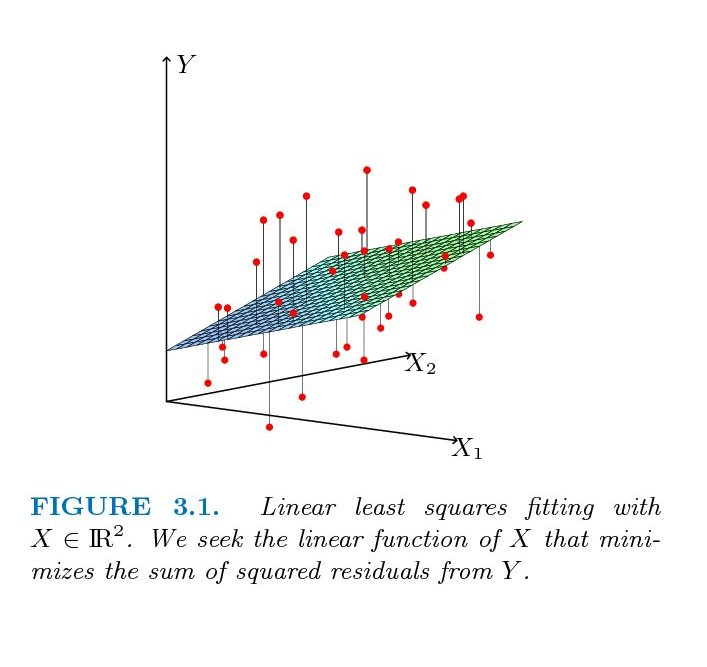
\includegraphics[scale=0.1]{images/figures3-0.jpg}
\pitem Arrange them as rows in matrix X. $\mat{x_{1}\\ x_{2} \\ ..}$.
\pitem Columns of X, y are centered.
\pitem Solve: $X\gb \approx y$.
\pitem Assume feature vectors have norm 1. \red{$XDD^{-1}\gb \approx y$}
\end{itemize}
\end{frame}

\begin{frame}
\frametitle{Shrinkage methods}
\begin{itemize}
\pitem Ridge regression.
\pitem Lasso.
\pitem Other penalties.\\
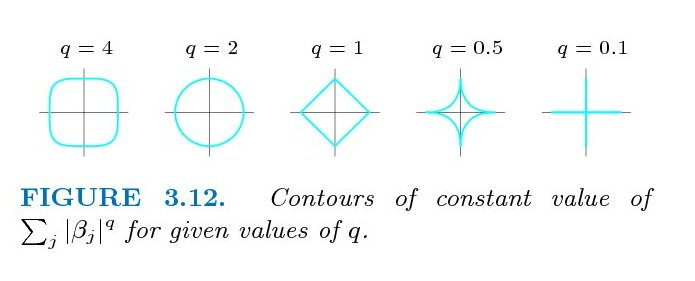
\includegraphics[scale=.25]{images/figures3-11.jpg}
\pitem Least angle regression.
\end{itemize}
From: \cite{hastie-elements}, \cite{hastie-lars}.

\end{frame}


\section{Least Angle regression}
\begin{frame}
\frametitle{Forward selection}
\begin{itemize}
\pitem Want sparse solution.
\pitem How to balance love of sparsity with desire for a good fit?
\end{itemize}
\end{frame}

\begin{frame}
\frametitle{Classical Forward Stepwise Selection}
\begin{itemize}
\pitem Init: $\gb = 0, A = \gf$.
\pitem Current fit: $\hat{\mu} = X \beta$. Residue: $r = y - \hat{\mu}$. Current set of features: A.
\pitem Grow A one feature at a time: Select $x_j = argmax_i\{\dprod{x_i, r}\}$. \\
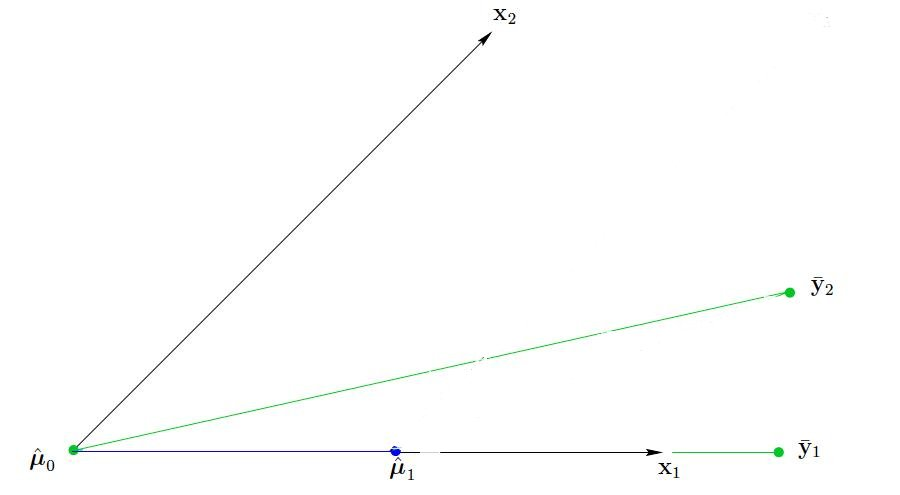
\includegraphics[scale=.2]{images/ForwardSelectionExample.jpg}
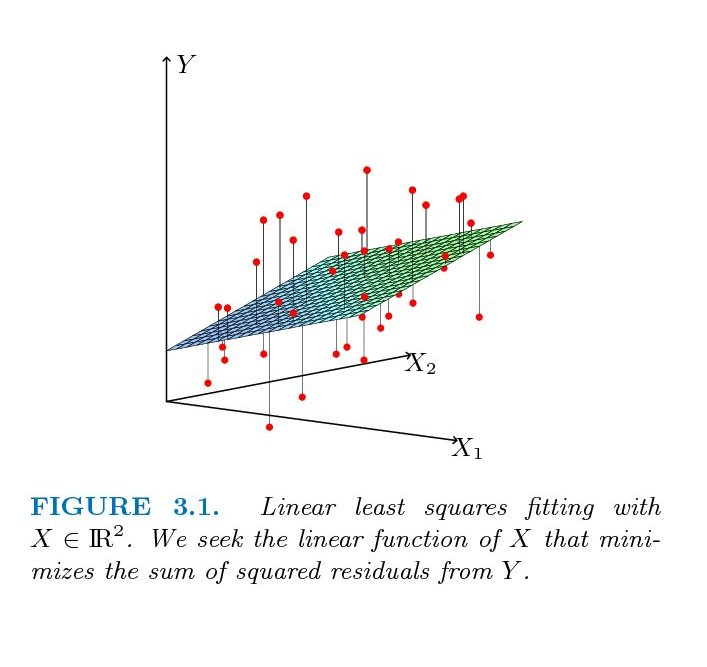
\includegraphics[scale=0.1]{images/figures3-0.jpg}
\end{itemize}
\end{frame}

\begin{frame}
\frametitle{LAR Algorithm}
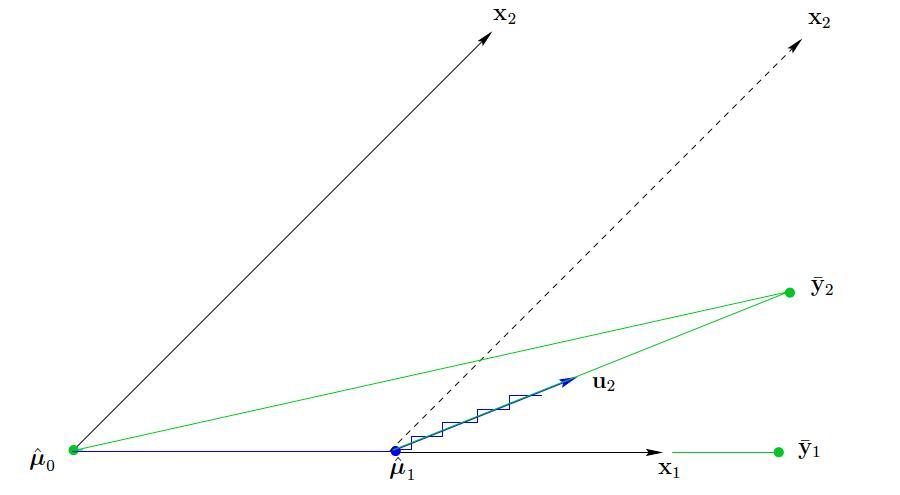
\includegraphics[scale=.2]{images/LARSimpleExample.jpg}
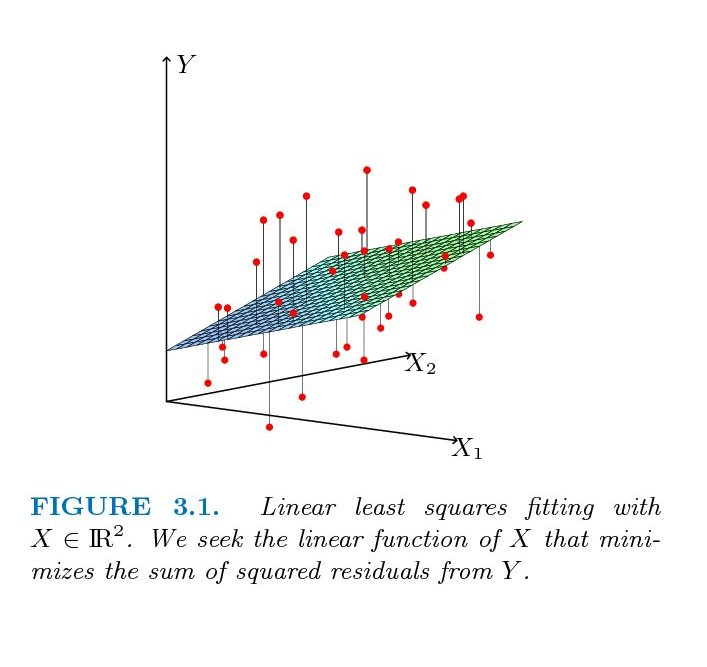
\includegraphics[scale=0.1]{images/figures3-0.jpg}
\begin{itemize}
\pitem Project residue r on subspace(A), get $u_i$.
\pitem Set $\gb_{A} = \gb_{A} + \gamma_i$.\\
So, $\mu = X\gb$ increases along $u_i$\\
until you find \red{${x_k} : \dprod{x_k, r} = \dprod{x_j, r}$}.
\pitem $A = A \union \set{x_k}$.
\pitem \red{Note!} At any point, the residue makes same angle with all $x_{i} \in A$.
% \\ 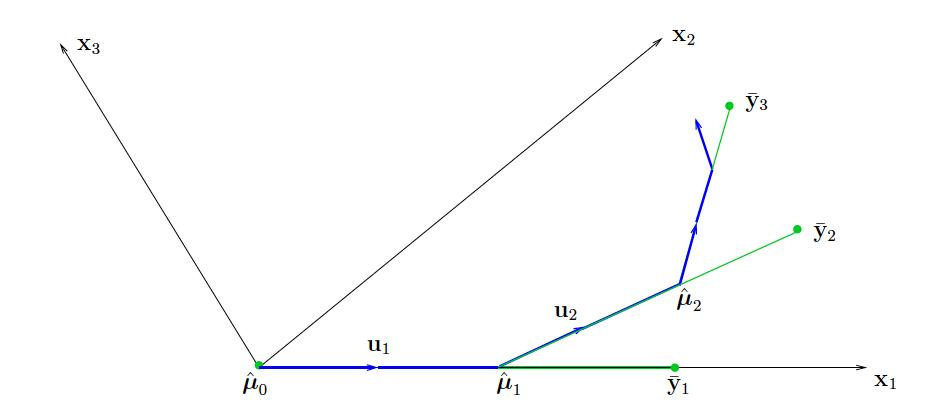
\includegraphics[scale=.25]{images/LARGeneralExample.jpg}
\end{itemize}
\end{frame}


\begin{frame}
\frametitle{See how the correlation evolves}
\begin{itemize}
\pitem $\hat{c}(\gb)$: the vector of correlations of the residue with $\set{x_{i}}$\\
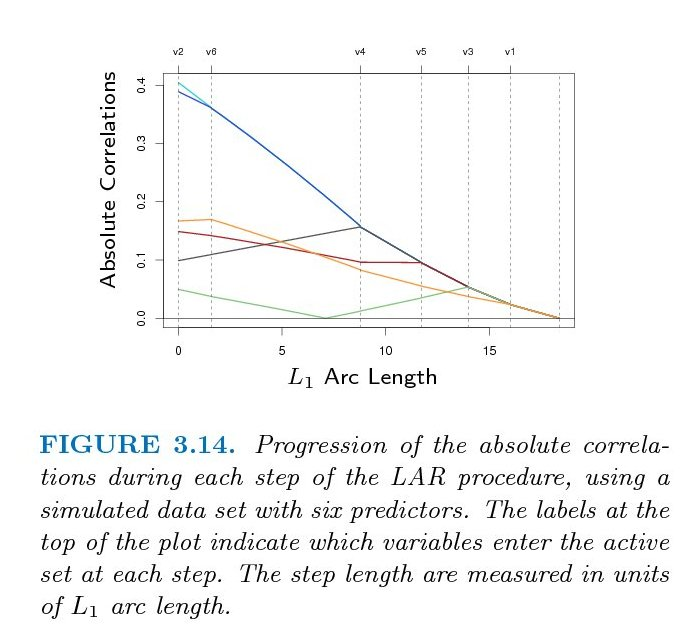
\includegraphics[scale=0.25]{images/figures3-13.jpg}
\end{itemize}
\end{frame}

\begin{frame}
\frametitle{Improvement over forward stepwise (greedy)}
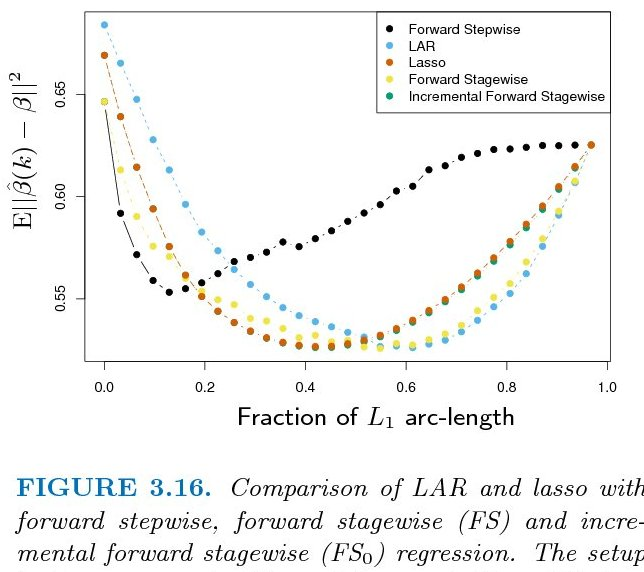
\includegraphics[scale=.25]{images/figures3-15.jpg}
\\How to balance love of sparsity with desire for a good fit?
\end{frame}

\section{LAR and Lasso: the connection}
\subsection{Lasso}
\begin{frame}
\frametitle{The objective}
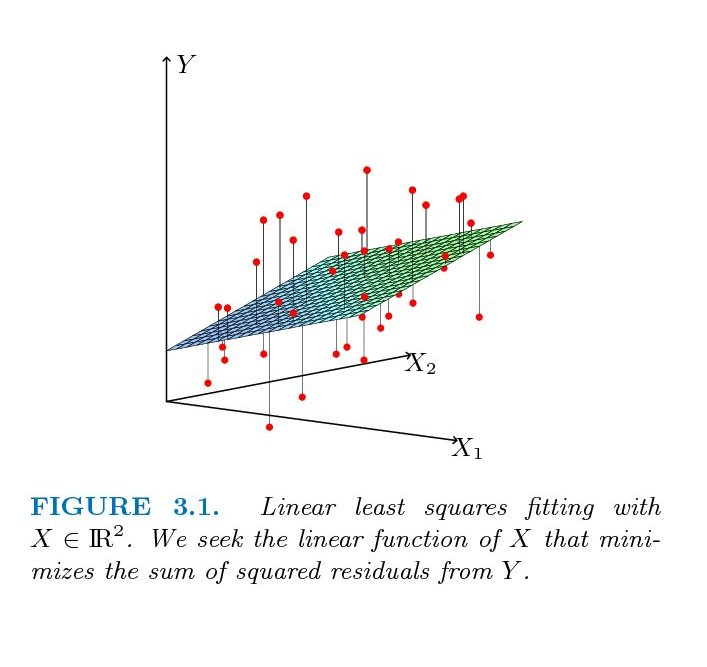
\includegraphics[scale=0.25]{images/figures3-0.jpg}
\begin{itemize}
\pitem $\hat{\gb} = argmin_{\gb} \norm{y-X\gb}_{2}^{2}$ subject to \red{$\sum |\gb_{i}| \leq t$}.
\pitem Same as $f(\hat{\gb}) = \min_{\gb} \norm{y-X\gb}_{2}^{2}$ \red{$+ \gl \sum_{i} |\gb_{i}|$}.
\end{itemize}
\end{frame}

\begin{frame}
\frametitle{Lasso for sparsity}
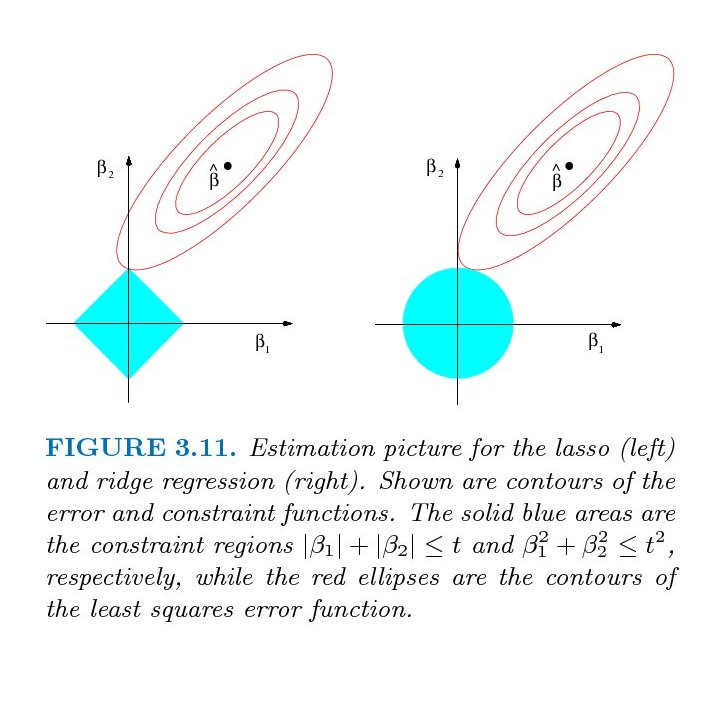
\includegraphics[scale=0.15]{images/figures3-10.jpg}
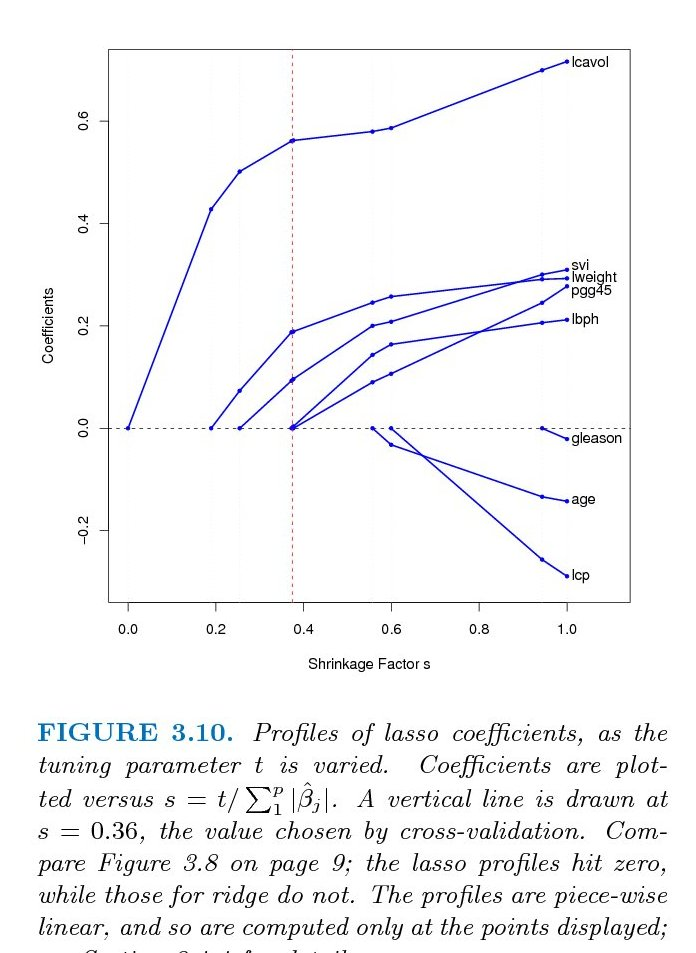
\includegraphics[scale=0.15]{images/figures3-9.jpg}
\\
$\hat{\gb} = argmin_{\gb} \norm{y-X\gb}_{2}^{2}$ subject to \red{$\sum |\gb_{i}| \leq t$}.
\begin{itemize}
\pitem \red{Quiz:} What t will reduce the problem to least squares?
\pitem \red{$t = \sum |\gb_{i}^{*}|$}.
\end{itemize}
\end{frame}

\subsection{The connection}
\begin{frame}
\frametitle{LARS: Solving LAR with Lasso}
\begin{itemize}
\pitem Experimental observation\\
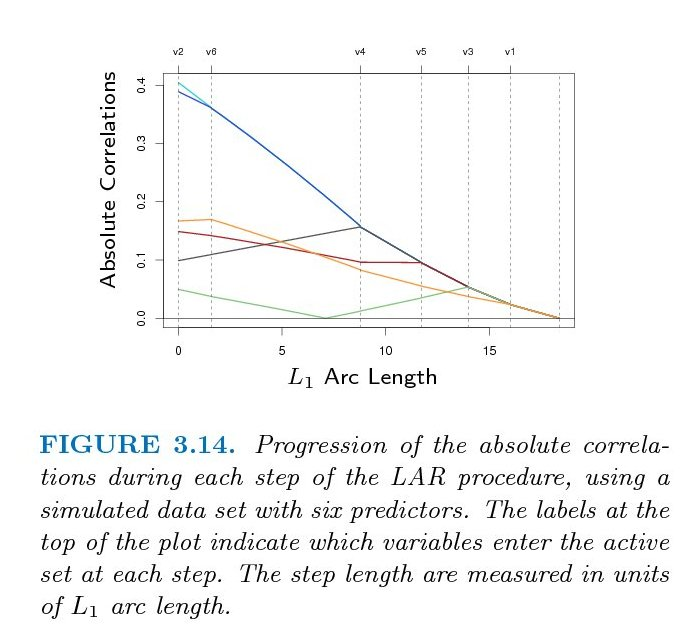
\includegraphics[scale=0.15]{images/figures3-13.jpg}
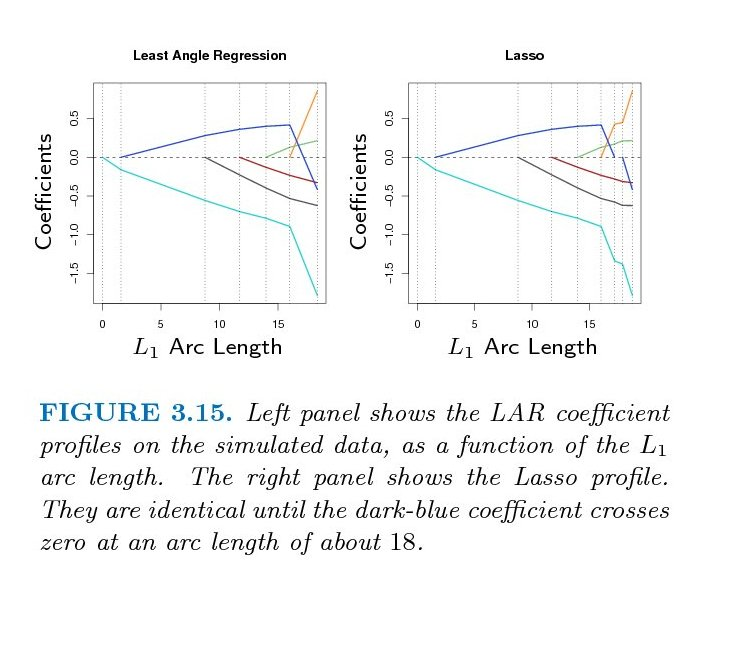
\includegraphics[scale=0.20]{images/figures3-14.jpg}
\pitem So $|\gb_{j}|$ can begin to decrease, and it can change sign.
\pitem The \red{LARS} fix: Drop coefficients which hit 0 out of 'active set'.
\end{itemize}
\end{frame}

\begin{frame}
\frametitle{Lasso solutions: Observations}
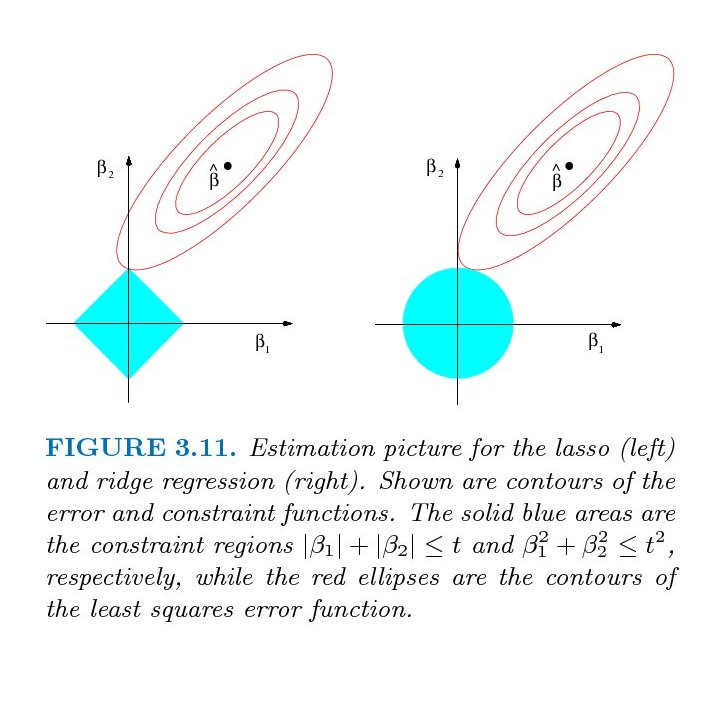
\includegraphics[scale=0.1]{images/figures3-10.jpg}
\begin{itemize}
\pitem Note: $f(\hat{\gb}) = \min_{\gb} \norm{y-X\gb}_{2}^{2}$ \red{$+ \gl \sum_{i} |\gb_{i}|$}.
\pitem Set $\gradient f(\gb) = 0$.
\pitem B := features in sparse solution.
\pitem Get conditions:
\\ $\forall j\in B: x_{j}^{T}(y-X\gb) = \gl *sgn(\gb_j)$.
\\ $\forall j\notin B: x_{j}^{T}(y-X\gb) = \gl *sgn(\gb_j) \leq |\gl|$.
\pitem \red{Remarkable!} $\gl \to $ upper bound on \blue{correlation} of the \blue{residue with $x_{j}$}.\\
\end{itemize}
\end{frame}

\begin{frame}
\frametitle{Compare with LAR}
\begin{itemize}
\pitem $\hat{c}$: correlation of residue with features. $s_j$: sign of correlation with feature j.
\pitem $\forall j\in A: x_{j}^{T}(y-X\gb) = \hat{c} * s_j$.
\pitem $\forall j\notin A: x_{j}^{T}(y-X\gb) \leq \hat{c}$.
\pitem Compare:
\\ $\forall j\in B: x_{j}^{T}(y-X\gb) = \gl *$ \red{$sgn(\gb_j)$}.
\\ $\forall j\notin B: x_{j}^{T}(y-X\gb) \leq |\gl|$.
\pitem When \red{$sgn(\gb_j)\neq s_j$}, Lasso $\neq$ LAR.
\pitem The \red{LARS} fix: If $\gb_{j}$ hits 0 for $j \in A$, it is about to change sign.
\end{itemize}
\end{frame}

\begin{frame}
\frametitle{When \red{$sgn(\gb_j)\neq s_j$}, Lasso $\neq$ LAR}
\begin{itemize}
\pitem Experimental observation\\
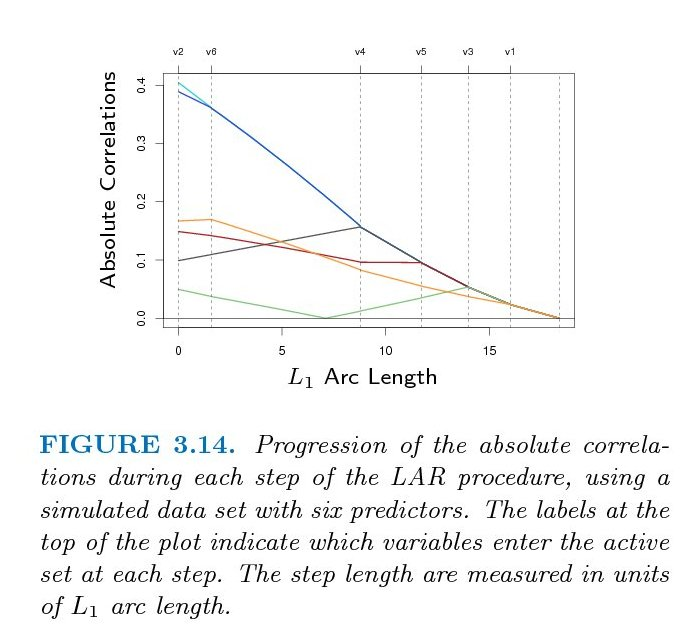
\includegraphics[scale=0.15]{images/figures3-13.jpg}
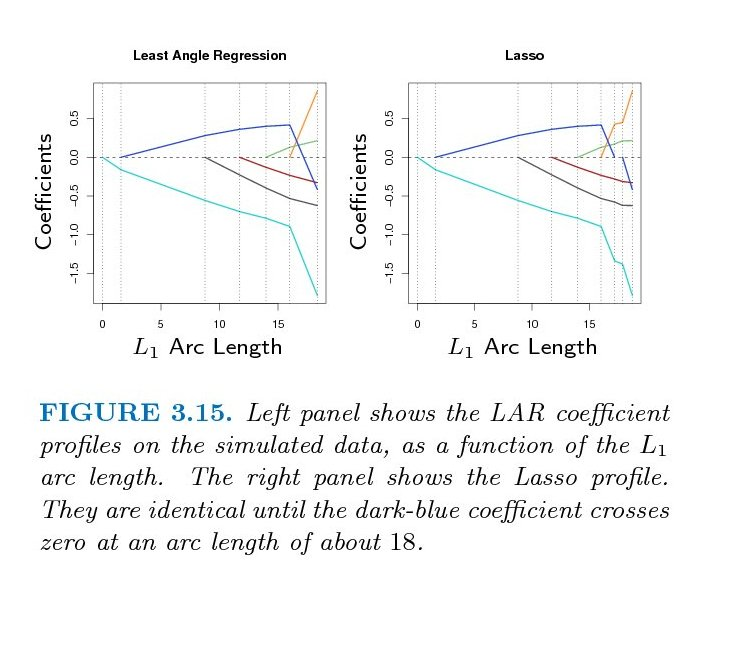
\includegraphics[scale=0.20]{images/figures3-14.jpg}
\pitem Geometric intuition: When does a coefficient start decreasing, even when correlation is positive? When you add feature v1 which is not independent of A. As $\gb_1 \up, \gb_6 \down$.
\end{itemize}
\end{frame}

\section{Conclusion}
\begin{frame}
\frametitle{What did we learn?}
\begin{itemize}
\pitem Least Angle regression (\red{LAR}): get sparse solutions, like forward stepwise regression; but modified to be non greedy.
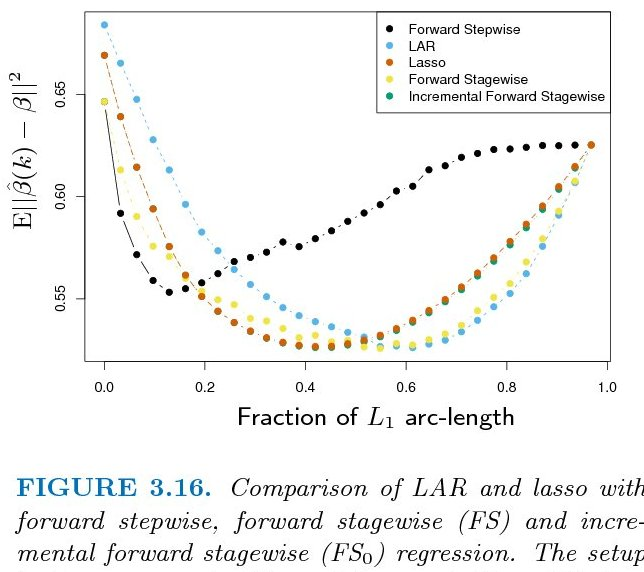
\includegraphics[scale=.1]{images/figures3-15.jpg}
\pitem \red{Lasso} for sparse solutions.
\pitem The sparse solutions are sometimes different.
\pitem \red{LARS}: LAR modified to solve Lasso. \red{Very efficient!} Also looked at how Lasso works with new eyes \red{$\bigstar \bigstar$}.
\end{itemize}
\end{frame}

\begin{frame}
\frametitle{References}
\bibliographystyle{plain}
\bibliography{../../statistics/statistics}
\end{frame}


\begin{frame}
\frametitle{Bye!}
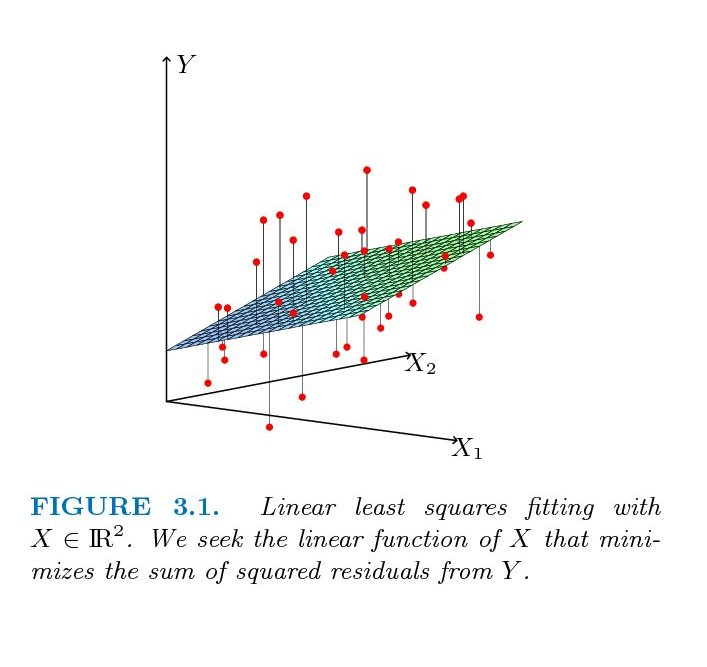
\includegraphics[scale=.25]{images/figures3-0.jpg}
\pause \\\red{Ask us some questions!}
\end{frame}



\end{document}
